\documentclass[aspectratio=169]{beamer}
%% Choose aspect ratio:
% [aspectratio=43]  % 4:3 (default)
% [aspectratio=169] % 16:9, wide


\usetheme[minimal,]{tugraz2018}
%% Choose main theme variant:
% [standard]        % standard (default)
% [institute]       % with institute's graphical acronym on the left
% [minimal]         % with reduced visuals

%% Choose your font style:
%                   % Helvetica (default for Corporate Design)
% [webfont]         % Source Sans Pro (as used on tugraz.at)
% [nofont]          % no font loaded - Computer Modern Sans

%% Choose your department's color instead of TU Graz red (optional):
% [arch]            % 
% [bau]             %
% [etit]            %
% [mbww]            %
% [tcvp]            %
% [mpug]            %
% [infbio]          %


\usepackage[utf8]{inputenc}
\usepackage[english]{babel}
\usepackage{pdfpages}
\usepackage{graphicx}
\usepackage{wasysym}
\usepackage{textcomp}
%% Choose your language:
% [ngerman]   % German
% [english]   % English


%% Add your own packages, macros, etc.
% ...


%% Enter presentation metadata
\title[Short Title]{JavaSQUIP}
\subtitle[Subtitle]{An implementation of a scheduler queue-based covert channel in JavaScript}
\author{Christoph Royer}
\date{ISW Presentations 12 Jan 2023}
\institute{IAIK}
\instituteurl{iaik.tugraz.at}

%% Logos
% \institutelogo{beamerthemetugraz/institute/kurz}  % graphical acronym for [institute] theme (left margin)
% \additionallogo{figures/logo}  % additional institute/department logo (footline; optional)
% \logobar{Supported by: ...}  % sponsors (titlepage; optional)


\begin{document}

\begin{frame}[plain]
  \maketitle
\end{frame}


\section{Introduction}

\begin{frame}{Networkless cross-browser communication}
  \centering
  \includegraphics[width=\textwidth]{figures/JSQUIP}
\end{frame}

\begin{frame}{AMD Zen2 Architecture}
\centering
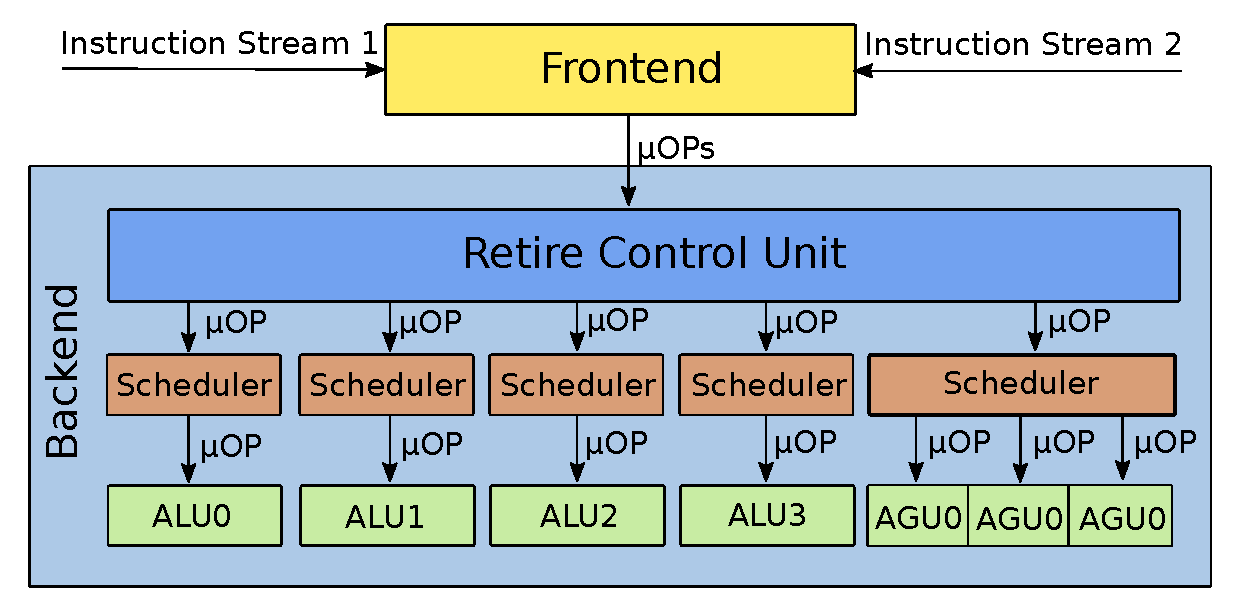
\includegraphics[page=1, width=0.7\textwidth]{figures/Zen2arch.pdf}

\tiny{cf. Software Optimization Guide for AMD EPYC 7002 Processors}
\end{frame}

\begin{frame}{Port contention}
\centering
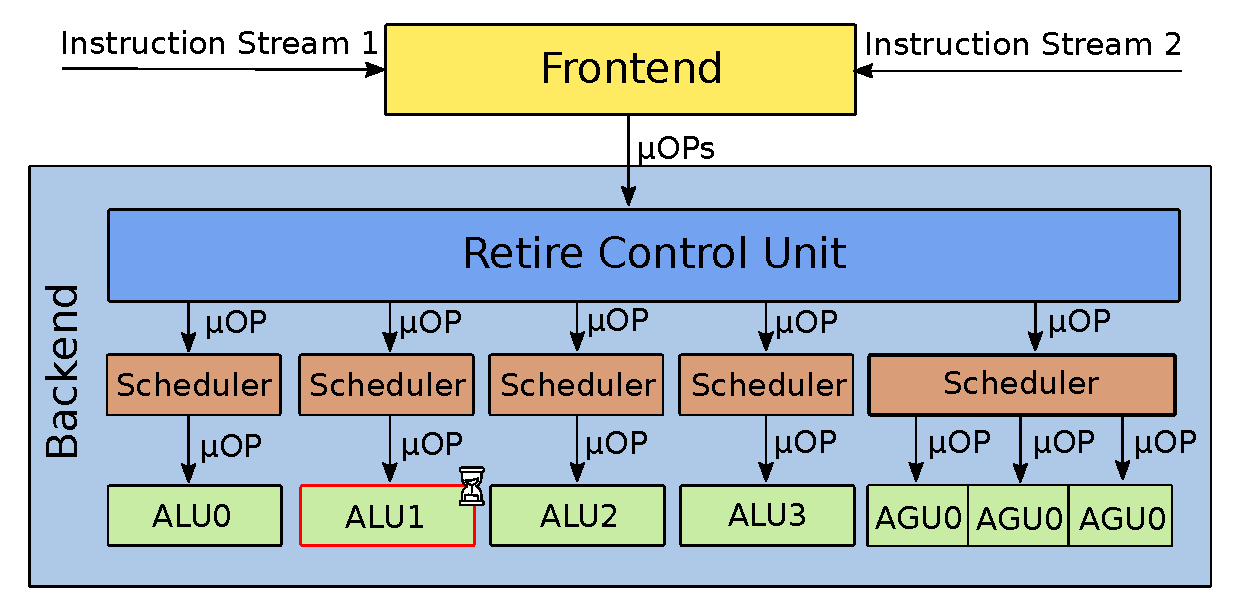
\includegraphics[page=1, width=0.7\textwidth]{figures/Zen2ALU.pdf}

\tiny{cf. Software Optimization Guide for AMD EPYC 7002 Processors}
\end{frame}


\begin{frame}{SQUIP: scheduler contention}
  \centering
  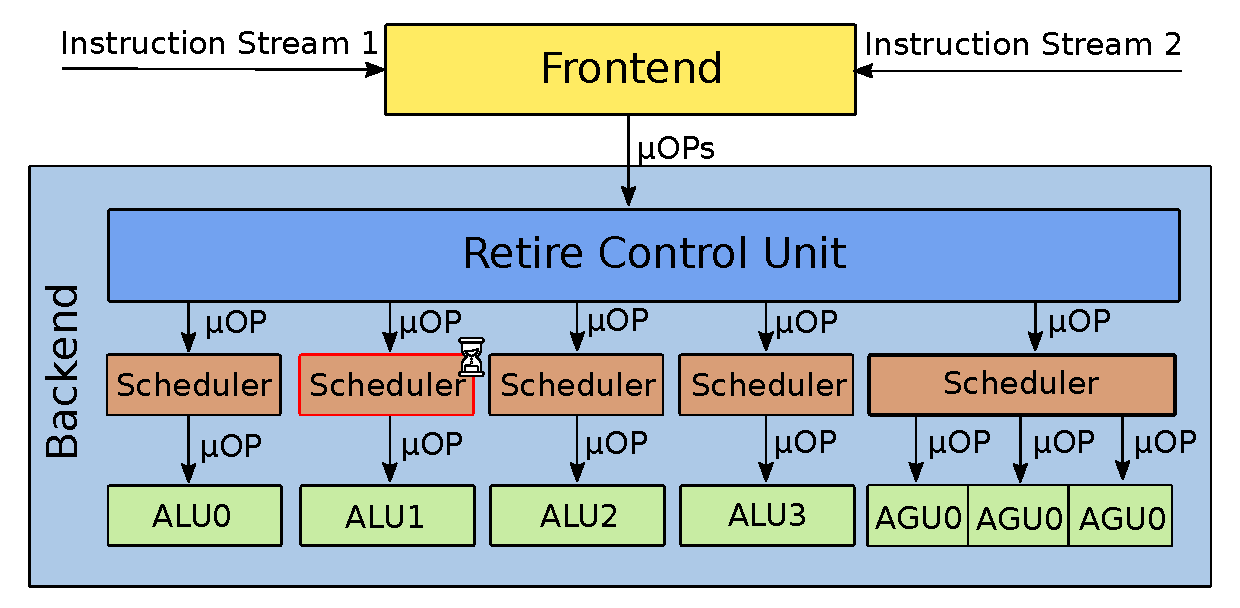
\includegraphics[page=1, width=0.7\textwidth]{figures/Zen2Scheduler.pdf}

  \tiny{cf. Software Optimization Guide for AMD EPYC 7002 Processors}
\end{frame}

\section{SQUIP in JavaScript}

\begin{frame}{Challenges}
  \begin{itemize}
    \item{colocation \visible<2->{\textrightarrow many Threads}}
    \item{accurate timing \visible<3->{\textrightarrow  counting thread}}
    \item{synchronisation \visible<4->{\textrightarrow  \texttt{DateTime.now()}}}
    \item{filling a scheduler \visible<5->{\textrightarrow  \texttt{Math.imul()}}}
  \end{itemize}
\end{frame}


\begin{frame}{JavaSQUIP: beating the competition 5-fold}
  \centering
  \includegraphics[width=\textwidth]{figures/JSQUIP}
\end{frame}

%\begin{frame}[c,plain]
\begin{frame}[c]
  \centering
  \Large Questions?
\end{frame}

\end{document}
